% Created 2019-05-10 Fri 17:26
% Intended LaTeX compiler: pdflatex
\documentclass[12pt, a4paper]{report}
\usepackage[utf8]{inputenc}
\usepackage[T1]{fontenc}
\usepackage[czech, ]{babel}
\usepackage{graphicx}
\usepackage{grffile}
\usepackage{longtable}
\usepackage{float}
\usepackage{wrapfig}
\usepackage{rotating}
\usepackage[normalem]{ulem}
\usepackage{amsmath}
\usepackage{textcomp}
\usepackage{amssymb}
\usepackage{capt-of}
\usepackage[hidelinks]{hyperref}
\usepackage{csquotes}
\usepackage{tabularx}
\MakeOuterQuote{"}
\usepackage{setspace}
\onehalfspacing
\usepackage{titlesec}
\titleformat{\chapter}[display]{\normalfont\bfseries}{}{0pt}{\Huge}
\usepackage[backend=bibtex,citestyle=authoryear]{biblatex}
\addbibresource{~/OneDrive/Orgmode/Papers/references.bib}


\DeclareUnicodeCharacter{00A0}{~}
% \addbibresource{./references.bib} % pro pouziti lokalni slozky se zdroji
\author{Matěj Haša, Vít Chrubasík, Marek Štěpán}
\date{Květen 2019}
\title{Projekt: Státní maturita s Khan Academy\\\medskip
\large 
\includegraphics[width=\linewidth]{./images/skola_logo.png} Seminární práce}
\hypersetup{
 pdfauthor={Matěj Haša, Vít Chrubasík, Marek Štěpán},
 pdftitle={Projekt: Státní maturita s Khan Academy},
 pdfkeywords={},
 pdfsubject={},
 pdfcreator={Emacs 26.1 (Org mode 9.2.3)}, 
 pdflang={Czech}}
\begin{document}

\maketitle
\tableofcontents
\thispagestyle{empty}



\chapter{Úvod}
\label{sec:org3f72f3c}
V této seminární práci se budeme snažit co nejlépe aplikovat nabyté vědomosti, získané z hodin kurzu Projektové řízení A, které se týkají úvodní fáze projektu. V této fázi se především projekt plánuje, analyzuje a ověřuje se, jestli je proveditelný v kontextu našich možných zdrojů, efektivní etc. Z tohoto důvodu jsme práci rozdělili do několika kapitol, jak můžete vidět v obsahu v následující sekci. 

Náš fiktivní projekt má za cíl implementaci výukových materiálů pro českou státní maturitu do již existující online vzdělávací platformy Khan Academy. Jak už název napovídá, jedná se o online výukovou službu, dostupnou na internetové síti. V aktuálním řešení (Květen 2019) jsou dostupné kurzy z většiny vědních oborů jako např. matematiky, biologie, chemie, fyziky, historie etc. Khan Academy je dostupná i v českém jazyce. S kolegy bychom chtěli vytvořit projekt, jehož obsahem bude rozšíření výukových materiálů na verzi s českou jazykovou mutací a to o výukové materiály pro českou státní maturitu z matematiky.
\chapter{Identifikační listina}
\label{sec:org8360286}
V této kapitole můžete shlédnout identifikační listinu, kterou jsme vytvořili za účelem uceleného přehledu o našem projektu. V listině jsme uvedli všechny klíčové parametry jako jasně definovaný cíl a účel projektu, rozdělení zodpovědností či milníky průběhu projektu, které nám budou jasně indikovat, že je čas měřit a ověřit část dosavadních výsledků projektu.

\begin{table}[htbp]
\caption{\textbf{Identifikační listina projektu}}
\centering
\footnotesize
\begin{tabularx}{\textwidth}{lX}
\textbf{Název projektu:} & Státní maturita s Khan Academy\\
\textbf{Obsah:} & Přidání přípravných kurzů ke státní maturitní zkoušce z matematiky do platformy Khan Academy\\
\textbf{Účel:} & Poskytnutí možnosti kvalitní přípravy ke státní maturitní zkoušce z matematiky\\
\textbf{Cíle projektu:} & 1. Zavést plnohodnotný kurz do již existující platformy, jehož výstupem bude člověk schopný úspěšně vykonat státní maturitní zkoušku z matematiky\\
 & 2. Zvýšit úspěšnost u maturitní zkoušky za matematiky\\
 & 3. Motivovat účastníky kurzu k dalšímu studiu, které zahrnuje matematiku\\
\textbf{Termín zahájení:} & Leden 2020\\
\textbf{Termín ukončení:} & Září 2021\\
\textbf{Vedoucí projektu:} & Vít Chrubasík\\
\textbf{Členové projektového týmu:} & Matěj Haša, Marek Štěpán\\
\textbf{Garant:} & Vít Chrubasík\\
\textbf{Milníky:} & 1. Vytvoření osnovy reflektované z oficiální osnovy uveřejněné Ministerstvem školství\\
& 2. Vypracování studijních materiálů\\
& 3. Implementace do již existující platformy KhanAcademy\\
\textbf{Vydáno:} & Květen 2019\\
\end{tabularx}
\end{table}


\chapter{Logický rámec}
\label{sec:org801389c}

\begin{table}[htbp]
\caption{\textbf{Logický rámec}}
\centering
\footnotesize
\begin{tabularx}{\textwidth}{|X|X|X|X|}
\hline
Sloupec intervencí & Objektivně měřitelný ukazatel & Zdroje informací k ověření & Rizika / předpoklady (vnější)\\
\hline
Zvýšit úspěšnost u státní maturity z matematiky & Absolventi kurzu & Dotazníky, výsledky absolventů & \\
\hline
Poskytnutí možnosti dobré přípravy ke zkoušce & Absolventi kurzu & Statistické údaje & Správně sestavený kurz, který se osvědčil v dobré přípravě studentů\\
\hline
Sekce Maturita na na české Khan Academy & Beta-testování, testovací a  kontrolní skupina & reporty z testování & Validní testovací scénáře, úspěšná fáze testování, statisticky významné zlepšení testovací skupiny\\
\hline
Návrh, implementace, testování, nasazení, údržba & Lidská práce, know-how, hardware, technologie, energie & Vedoucí pracovníci, road map, účetní výkazy & Správná analýza, kvalitní vývojová platforma, dobře fungující tým\\
\hline
 &  &  & Svolení k realizaci projektu ze strany Khan Academy\\
\hline
\end{tabularx}
\end{table}

\chapter{SWOT analýza}
\label{sec:org455a7dc}
Před samotnou realizací projektu jsme si sepsali naše silné a slabé stránky, příležitosti i hrozby. Vytvořili jsme analýzu SWOT. Jsme si vědomi faktu, že je v našich silách ovlivnit jak naše slabé tak silné stránky. Hrozeb je třeba se vyhnout.

V případě našeho projektu jednoznačné pozitivum vidíme v integraci našeho řešení do již zaběhlé a fungující platformy. Nejen, že tato služba má již své klienty, ale také IT řešení již má fungující platformu. Budeme nabízet veřejně prospěšnou činnost, což se v dněšní době sociálně marketingové koncepce nosí. Lidé zkrátka slyší na produkty, jejichž zájem je sladěn s dlouho\-dobými sociálními a etickými zájmy celé společnosti. Služba je na českém trhu originální. Existují youtubeři a domácí lektoři, kteří se snaží připravovat studenty na úspěšné zvládnutí maturitní zkoušky z matematiky, ale nikdo nenabízí komplexní řešení krok po kroku, jako my.

Slabé stránky vidíme v našem týmu, který je poměrně malý a nezkušený. Ani jeden z nás nemá zkušenosti s podobným projektem. Ruku v ruce s tímto tvrzením jde i malý rozpočet, který především v pozdějších fázích projektu může být problém a výsledný produkt se může začít ochuzovat o potřebné fáze jako např. důsledné testování. Budeme se snažit náš tým přetransformovat z nezkušených nováčků na tomto trhu na inovativní skupinu, která může přinést nové nápady či řešení v odvětví online vzdělávání.

Když přijde na příležitosti našeho projektu, myslíme si, že vzhledem ke jeho dobrým účelům, o kterých jsme hovořili v silných stránkách, může chtít přispět k vývoji řada dobrovolníků. Také budeme aktivní na poli žádostí o dotace. 

Po důkladné analýze jsme vyčlenili čtyři nejzávažnější hrozby. Mohou přijít změny ze strany Ministerstva školství a to jak v aktuálních osnovách maturity tak v úplném zrušení státní maturitní zkoušky. Této hrozbě nijak předejít nejde, pravděpodobnost zrušení státní zkoušky je naštěstí malá. Změnit osnovy se mohou a na tuto hrozbu jsme připraveni --- budeme iterativně kontrolovat oficiální požadavky na studenty a na jejich základě pružně reagovat na potenciální změny. Samozřejmě i nám se nevyhne riziko možných konkurenčních bojů, ale spolu s kolegy se této skutečnosti neobáváme. Khan Academy si drží značnou část trhu a nic nenaznačuje změnám v blízké budoucnosti. Může se stát, že top management Khan Academy s námi odmítne spolupracoavt --- budeme se snažit projekt uvést v co možná nejlepším světle, abychom tuto hrozbu snížili na minimální hodnotu.

Pro ucelený přehled můžete nahlédnout v tabulce \ref{tab:swot}.

\begin{table}[htbp]
\caption{\label{tab:swot}
\textbf{SWOT analýza}}
\centering
\footnotesize
\begin{tabularx}{\textwidth}{|X|r|r|r|}
\hline
Položka & Váha & Hodnocení & Hodnota\\
\hline
\textbf{Silné stránky} &  &  & \\
Materiálová nenáročnost & 10 & 2 & 0.2\\
Veřejně prospěšná činnost & 20 & 3 & 0.6\\
Originalita & 30 & 5 & 1.5\\
Implementace do zaběhnutého systému & 40 & 5 & 2.\\
\hline
\textbf{Silné stránky celkem} & 100 &  & 4.3\\
\hline
\textbf{Slabé stránky} &  &  & \\
Malý tým & 12 & 4 & -0.48\\
Nově sestavený tým & 20 & 1 & -0.2\\
Nizký rozpočet & 33 & 2 & -0.66\\
Málo praktických zkušeností & 35 & 3 & -1.05\\
\hline
\textbf{Slabé stránky celkem} & 100 &  & -2.39\\
\hline
\textbf{Příležitosti} &  &  & \\
Dotace & 25 & 2 & 0.5\\
Dobrovolníci & 47 & 4 & 1.88\\
Zvýšení poptávky & 12 & 1 & 0.12\\
Nefinanční příspěvky & 16 & 3 & 0.48\\
\hline
\textbf{Příležitosti celkem} & 100 &  & 2.98\\
\hline
\textbf{Hrozby} &  &  & \\
Změní se osnovy maturity & 35 & 3 & -1.05\\
Konkurence & 6 & 1 & -0.06\\
Odmítnutí návrhu implementace & 40 & 3 & -1.2\\
Zrušení státní maturity & 19 & 1 & -0.19\\
\hline
\textbf{Hrozby celkem} & 100 &  & -2.5\\
\hline
\textbf{Interní faktory} &  &  & 1.91\\
\textbf{Externí faktory} &  &  & 0.48\\
\hline
\textbf{Závěr} &  &  & \textbf{2.39}\\
\hline
\end{tabularx}
\end{table}

\chapter{Myšlenková mapa}
\label{sec:orgcabfeb6}
\begin{figure}[htbp]
\centering
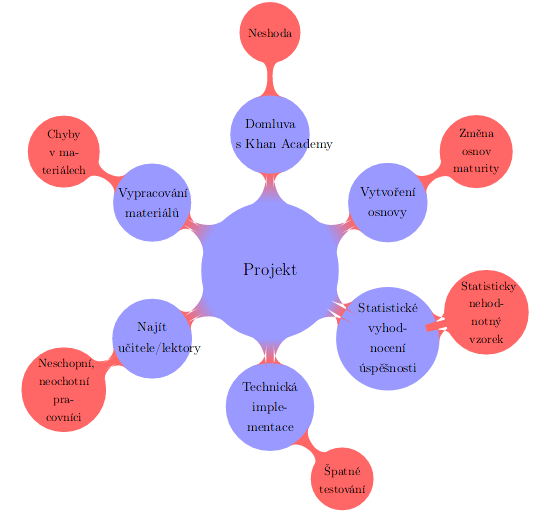
\includegraphics[width=.9\linewidth]{./images/myslenkova_mapa.png}
\caption{\label{fig:myslenkova_mapa}
Myšlenková mapa}
\end{figure}



\chapter{MS Project}
\label{sec:org4918916}

\texttt{odkaz na ms project}

Provedení projektu bylo rozděleno na 6 etap. Po sestavení a zaškolení týmu se začne paralelně pracovat na vytváření osnovy a softwarové integraci do existující platformy. Jakmile budou tyto etapy dokončeny, začne testovací fáze s testovací skupinou, která bude následována vyhodnocením.

\begin{itemize}
\item Sestavení týmu
\item Vytvoření osnovy
\item Vypracování studijních materiálů
\item Integrace do platformy Khan Academy
\item Testovací fáze
\item Vyhodnocení projektu
\end{itemize}

\begin{center}
\begin{tabular}{r}
0.58333333\\
\end{tabular}
\end{center}

\section{Kritická cesta}
\label{sec:org5e23070}
Projekt obsahuje celkem 36 činností, z toho 21 jich bylo identifi\-kováno jako kritických \(\implies\) index kritičnosti vychází na \textbf{58,33 \%.} Toto číslo přesahuje hranici proveditelnosti, a proto bude třeba v plánu provést další opatření.
% jaká opatření

\section{Stakeholdeři}
\label{sec:orge5816cf}
\begin{table}[htbp]
\caption{\textbf{Seznam stakeholderů a jejich vlivů}}
\centering
\footnotesize
\begin{tabularx}{\textwidth}{lX}
Vedoucí projektu & \\
Liniový management & \\
Týmoví pracovníci & \\
Studenti & \\
Externisté & \\
\end{tabularx}
\end{table}


\chapter{Budoucí vývoj}
\label{sec:org2ad0c11}
Možnost budoucího vývoje vidíme v rozšíření přípravy i pro jiné předměty státní české maturitní zkoušky. Jako iniciátoři projektu máme všichni matematiku rádi a zároveň má tento předmět jedny z nejhorších úspěšnostních výsledků -- z tohoto důvodu jsme se rozhodli připravovat studenty právě pro matematiku. Do budoucna se však nebráníme rozšířit řešení i o Český jazyk, Anglický jazyk a další, třeba i odborné předměty.

Je samozřejmostí, že pro další rozšíření aplikace mimo obor matematiky bychom museli využít více externích pracovních sil z důvodu naší nedostatečné znalosti. Zdali navážeme dalším projektem či dokonce projekty bude záležet na úspěšnosti provedení tohoto, vyjednání podmínek s Khan Academy a oblíbenosti budoucí služby obecně.

V daleké budoucnosti vidíme možnost i ve vzdělávání a přípravě na certifikáty a kurzy obecně. Existují kurzy angličtiny jako např. FCE, certifikáty pro přehled o testování software ISTQB a jistě plno dalších z mnoha oborů. Většinou již existují přípravné knihy jak fyzické tak elektronické, ale těžko se vyrovnají vedenému digitálnímu průvodci, který studenta vede krok po kroku a vše důsledně vysvětluje. Student má také snadno dostupné diskusní fórum, kde případné problémy může okamžite konzultovat se svými kolegy. Z tohoto důvodu si myslíme, že výše zmíněné navázání by za jistých okolnosti určitě mělo smysl.
\chapter{Závěr}
\label{sec:org6851c0b}
\end{document}